\documentclass[a4paper]{article}
\usepackage{amsmath}
\usepackage{amsfonts}
\usepackage{tikz}
\usepackage{tkz-graph}
\usepackage{mathtools}
\usepackage{tabularx}
\usepackage{graphicx}
\usepackage{blkarray}
\usepackage{booktabs} 
\graphicspath{ {./figures/} }


\title{Optimal accuracy threshold using 0-1 ILP formulation}
\date{}
\author{Dr. Pouria Ramazi, Arash Mari Oriyad}

\usepackage[utf8]{inputenc}
\usepackage{fourier, heuristica}
\usepackage[colorlinks=true]{hyperref}
\usepackage{array, ltablex, multirow} % tabularx: auf Textbreite vergrößern

\usepackage{makecell}
\setcellgapes{5pt}
\makegapedcells
\renewcommand\theadfont{\bfseries}
\renewcommand\cellalign{rc}


\begin{document}
\maketitle

\begin{abstract}
Classification 
\end{abstract}

For a binary classification problem, the accuracy measure which is the portion of the correctly predicted instances with respect to all instances, can be calculated as below,
\[
accuracy = \frac{TP + TN}{TP + TN + FP + FN}
\]
where $TP$, $TN$, $FP$, and $FN$ are the number of true-positive, true-negative, false-positive, and false-negative instances, respectively.

While accuracy requires the predicted labels, classification models produce a probability distribution over all available classes for each instance. Hence, one must apply a threshold to the predicted probabilities to obtain deterministic labels. An optimal threshold for a given set of instances is a real value between 0 and 1, providing the highest accuracy.

A trivial approach to determine such a threshold is an exhaustive search that examines all the possible threshold values to obtain the best one. Complete search-based methods are usually not efficient in execution time, especially when the solution space grows. To the best of our knowledge, there is no programming package to find the optimal accuracy threshold without using an exhaustive search.

We treated the optimal accuracy threshold problem as an optimization problem by introducing an integer linear programming (ILP) formulation. Assume a set of $N$ instances with a binary target variable $y$ and suppose $\hat{y_i}$ is the predicted probability for the $i$th instance. Then, $\tilde{y_i}$ is a binary decision variable which is desirable to be calculated as follows:

\[
\tilde{y_i} = 
\begin{cases}
0, & \hat{y_i} < t \\
1, & \hat{y_i} \ge t
\end{cases}
\]

where $t$ is the threshold. More precisely, $\tilde{y_i}$ represents the label of $i$th instance after applying the threshold $t$ to the predicted probability $\hat{y_i}$. Hence, the accuracy measure can be calculated as bellow.

\[
accuracy = 1 - \frac{1}{N} \sum_{i=1}^{N} |y_i - \tilde{y_i}|
\]

Put them all together, the following optimization formulation is achieved.

\begin{equation}
\begin{aligned}
	&\text{minimize} \quad \sum_{i=1}^{N} |y_i - \tilde{y_i}| \\
	&\text{subject to:} \quad \tilde{y_i} = 
	\begin{cases}
	0, & \hat{y_i} < t \\
	1, & \hat{y_i} \ge t
	\end{cases} \qquad \forall 1\le i \le N\\
	& \qquad \qquad \qquad \tilde{y_i} \in \{0, 1\} \qquad \forall 1\le i \le N
\end{aligned}
\end{equation}

Note that $y_i$ and $\hat{y_i}$ are input parameters and $\tilde{y_i}$ is the decision variable of the problem. Moreover, $\frac{1}{N}$ is ignored in the objective function since $N$ does not affect the final solution.

To transform the proposed constraints into a linear form, for each $i$, we can combine the conditions and replace them with two new constraints. Similarly, to make the objective function linear, a new binary decision variable $z_i=|y_i - \tilde{y_i}|$ is defined and two new constraints are added to the optimization formulation as follows:

\begin{equation}
\begin{aligned}
&\text{minimize} \quad \: \: \: \: \sum_{i=1}^{N} z_i \\
&\text{subject to:} \quad \: \: z_i \ge y_i - \tilde{y_i} \qquad &\forall 1\le i \le N\\
& \qquad \qquad \qquad z_i \ge \tilde{y_i}  - y_i \qquad &\forall 1\le i \le N\\
& \qquad \qquad \qquad \hat{y_i} (1 - \tilde{y_i}) < t \qquad &\forall 1\le i \le N\\
& \qquad \qquad \qquad  \tilde{y_i} (\hat{y_i} - 1) \ge t - 1 \qquad &\forall 1\le i \le N\\
& \qquad \qquad \qquad \tilde{y_i} \in \{0, 1\} \qquad &\forall 1\le i \le N \\
& \qquad \qquad \qquad 0 \le t \le 1
\end{aligned}
\end{equation}

Hence, we have designed a 0-1 ILP formulation with $2N$ binary decision variables and $4N$ linear constraints.

The proposed ILP formulation is compared with the exhaustive search method in terms of average execution time (Table 1).

\pagebreak

\begin{center}
\begin{tabularx}{1.2\textwidth}
	{ 
		| >{\centering\arraybackslash}X 
		| >{\centering\arraybackslash}X 
		| >{\centering\arraybackslash}X
		| >{\centering\arraybackslash}X
		| >{\centering\arraybackslash}X
		| >{\centering\arraybackslash}X
		|
	}
	\caption{Comparing the ILP-based approach with the exhaustive search method for finding the optimal accuracy threshold.}\label{tab:1}\\
	\hline
	\# Instances & Prediction Decimal & ILP (Python)& Exhaustive Search (Python) & ILP (C++) & Exhaustive Search (C++) \\
	\hline
	1000 & 1 & 0.032 & 0.025 & 0.0068 & 0.0024 \\
	\hline
	1000 & 2 & 0.150 & 0.199 & 0.067 & 0.0062\\
	\hline
	1000 & 3 & 1.133 & 1.243 & 0.802 & 0.028\\
	\hline
	1000 & 4 & 1.748 & 1.884 & 1.311 & 0.041\\
	\hline
	1000 & 5 & 1.807 & 1.860 & 1.339 & 0.045\\
	\hline
	2000 & 1 & 0.033 & 0.026 & 0.010 & 0.0042\\
	\hline
	2000 & 2 & 0.160 & 0.205 & 0.076 & 0.013\\
	\hline
	2000 & 3 & 2.747 & 1.721 & 2.152 & 0.076\\
	\hline
	2000 & 4 & 6.378 & 3.533 & 5.173 & 0.159\\
	\hline
	2000 & 5 & ? & ? & ? & 0.172\\
	\hline
	5000 & 1 & ? & ? & 0.023 & 0.010\\
	\hline
	5000 & 2 & ? & ? & 0.098 & 0.030\\
	\hline
	5000 & 3 & 5.998 & 2.075 & 5.060 & 0.234\\
	\hline
	5000 & 4 & ? & ? & ? & 0.875\\
	\hline
	5000 & 5 & 50.663 & 9.747 & ? & 1.091 \\
	\hline
	$10^{4}$ & 1 & ? & ? & 0.043 & 0.0216 \\
	\hline
	$10^{4}$ & 2 & ? & ? & 0.127 & 0.0634 \\
	\hline
	$10^{4}$ & 3 & ? & ? & 5.527 & 0.397 \\
	\hline
	$2 \times 10^{4}$ & 1 & ? & ? & 0.086 & 0.0421 \\
	\hline
	$2 \times 10^{4}$ & 2 & ? & ? & 0.179 & 0.130 \\
	\hline
	$2 \times 10^{4}$ & 3 & ? & ? & 6.227 & 0.818 \\
	\hline
	$5 \times 10^{4}$ & 1 & ? & ? & 0.212 & 0.115 \\
	\hline
	$5 \times 10^{4}$ & 2 & ? & ? & 0.314 & 0.330 \\
	\hline
	$5 \times 10^{4}$ & 3 & ? & ? & 7.115 & 2.059 \\
	\hline
	$10^{5}$ & 1 & ? & ? & 0.429 & 0.218 \\
	\hline
	$10^{5}$ & 2 & ? & ? & 0.539 & 0.642 \\
	\hline
	$10^{5}$ & 3 & ? & ? & 7.351 & 5.014 \\
	\hline
	$2 \times 10^{5}$ & 1 & ? & ? & 0.866 & 0.439 \\
	\hline
	$2 \times 10^{5}$ & 2 & ? & ? & 0.966 & 1.370 \\
	\hline
	$2 \times 10^{5}$ & 3 & ? & ? & 8.462 & 10.518 \\
	\hline
	$5 \times 10^{5}$ & 1 & ? & ? & 2.108 & 1.102 \\
	\hline
	$5 \times 10^{5}$ & 2 & ? & ? & 2.254 & 3.642 \\
	\hline
	$5 \times 10^{5}$ & 3 & ? & ? & 10.771 & 29.151 \\
	\hline
	$10^{6}$ & 1 & ? & ? & 4.131 & 2.229 \\
	\hline
	$10^{6}$ & 2 & ? & ? & 4.451 & 7.088 \\
	\hline
	$10^{6}$ & 3 & ? & ? & 13.010 & 60.555 \\
	\hline
	$2 \times 10^{6}$ & 1 & ? & ? & 8.198 & 4.703 \\
	\hline
	$2 \times 10^{6}$ & 2 & ? & ? & 8.692 & 17.500 \\
	\hline
	$2 \times 10^{6}$ & 3 & ? & ? & 17.751 & 166.988 \\
	\hline
\end{tabularx}
\end{center}

\pagebreak

\begin{center}
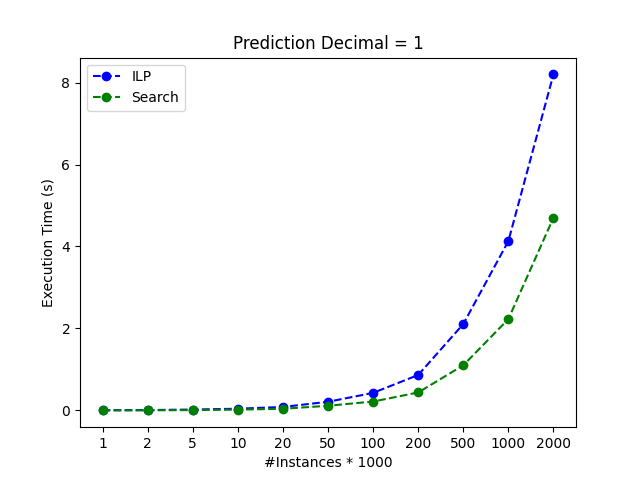
\includegraphics[]{figure_1}
\end{center}

\begin{center}
	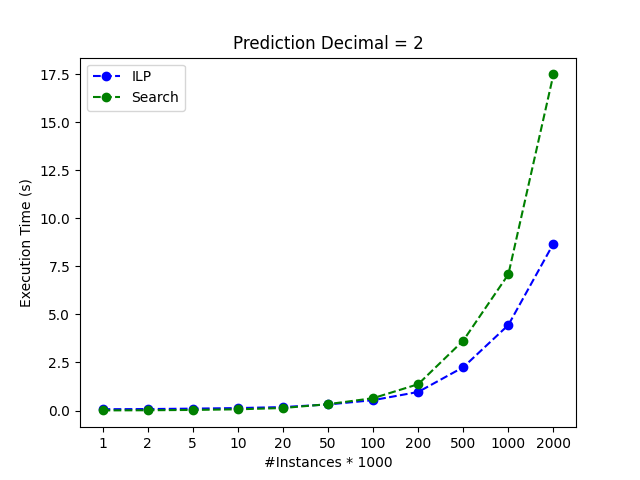
\includegraphics[]{figure_2}
\end{center}

\begin{center}
	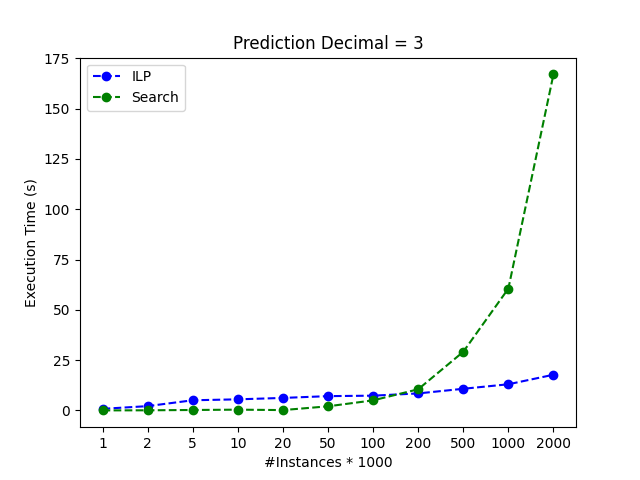
\includegraphics[]{figure_3}
\end{center}


\pagebreak

For $N=2$:
\begin{equation}
\begin{aligned}
&\text{minimize} \quad \: \: \: \: z_1 + z_2 \\
&\text{subject to:} \quad \: \: z_1 + \tilde{y_1}\ge y_1\\
&\qquad \qquad \qquad z_2 + \tilde{y_2}\ge y_2\\
& \qquad \qquad \qquad z_1 - \tilde{y_1} \ge - y_1\\
& \qquad \qquad \qquad z_2 - \tilde{y_2} \ge - y_2\\
& \qquad \qquad \qquad \hat{y_1}\tilde{y_1} + t \ge \hat{y_1} + \epsilon\\
& \qquad \qquad \qquad \hat{y_2}\tilde{y_2} + t \ge \hat{y_2} + \epsilon\\
& \qquad \qquad \qquad  (\hat{y_1} - 1)\tilde{y_1} - t \ge - 1\\
& \qquad \qquad \qquad  (\hat{y_2} - 1)\tilde{y_2} - t \ge - 1\\
\end{aligned}
\end{equation}


\begin{equation}
\begin{aligned}
&\text{minimize} \quad \: \: \: \: wx \\
&\text{subject to:} \quad \: \: Ax\ge b\\
\end{aligned}
\end{equation}


\[
A = \begin{blockarray}{ccccc}
z_1 & z_2 & \tilde{y_1} & \tilde{y_2} & t \\
\begin{block}{(cc|cc|c)}
1 & 0 & 1 & 0 & 0 \\
0 & 1 & 0 & 1 & 0 \\
\cmidrule{1-5}
1 & 0 & -1 & 0 & 0 \\
0 & 1 & 0 & -1 & 0 \\
\cmidrule{1-5}
0 & 0 & \hat{y_1} & 0 & 1 \\
0 & 0 & 0 & \hat{y_2} & 1 \\
\cmidrule{1-5}
0 & 0 & \hat{y_1}-1 & 0 & -1 \\
0 & 0 & 0 & \hat{y_2}-1 & -1 \\
\end{block}
\end{blockarray}_{8\times5}
\]


\[
x = \begin{blockarray}{c}
 \\
\begin{block}{(c)}
z_1 \\
z_2 \\
\cmidrule{1-1}
\tilde{y_1} \\
\tilde{y_2} \\
\cmidrule{1-1}
t \\
\end{block}
\end{blockarray}_{5\times1}
\]

\[
b = \begin{blockarray}{c}
\\
\begin{block}{(c)}
y_1 \\
y_2 \\
\cmidrule{1-1}
-y_1 \\
-y_2 \\
\cmidrule{1-1}
\hat{y_1} + \epsilon \\
\hat{y_2} + \epsilon \\
\cmidrule{1-1}
-1 \\
-1 \\
\end{block}
\end{blockarray}_{8\times1}
\]


\pagebreak


\[
A = \begin{blockarray}{ccccccccc}
z_1 & z_2 & \dots & z_N & \tilde{y_1} & \tilde{y_2} & \dots & \tilde{y_N} & t \\
\begin{block}{(cccc|cccc|c)}
1 & 0 & \dots & 0 & 1 & 0 & \dots & 0 & 0 \\
0 & 1 & \dots & 0 & 0 & 1 & \dots & 0 & 0\\
\vdots & \vdots & \ddots & \vdots & \vdots & \vdots & \ddots & \vdots & \vdots\\
0 & 0 & \dots & 1 & 0 & 0 & \dots & 1 & 0\\
\cmidrule{1-9}
1 & 0 & \dots & 0 & -1 & 0 & \dots & 0 & 0 \\
0 & 1 & \dots & 0 & 0 & -1 & \dots & 0 & 0\\
\vdots & \vdots & \ddots & \vdots & \vdots & \vdots & \ddots & \vdots & \vdots\\
0 & 0 & \dots & 1 & 0 & 0 & \dots & -1 & 0\\
\cmidrule{1-9}
0 & 0 & \dots & 0 & \hat{y_1} & 0 & 0 & 0 & 1 \\
0 & 0 & \dots & 0 & 0 & \hat{y_2} & 0 & 0 & 1\\
\vdots & \vdots & \ddots & \vdots & \vdots & \vdots & \vdots & \vdots & \vdots\\
0 & 0 & \dots & 0 & 0 & 0 & 0 & \hat{y_N} & 1\\
\cmidrule{1-9}
0 & 0 & \dots & 0 & \hat{y_1}-1 & 0 & 0 & 0 & -1 \\
0 & 0 & \dots & 0 & 0 & \hat{y_2}-1 & 0 & 0 & -1\\
\vdots & \vdots & \ddots & \vdots & \vdots & \vdots & \vdots & \vdots & \vdots\\
0 & 0 & \dots & 0 & 0 & 0 & 0 & \hat{y_N}-1 & -1\\
\end{block}
\end{blockarray}_{4N\times (2N+1)}
\]

\pagebreak

\[
recall = \frac{TP}{TP+FN} = \frac{TP}{\text{\# class 1}}
\]

\begin{equation}
\begin{aligned}
&\text{maximize} \quad \: \: \: \: \sum_{i=1}^{N} y_i \tilde{y_i} \\
& \qquad \qquad \qquad \hat{y_i} (1 - \tilde{y_i}) < t \qquad &\forall 1\le i \le N\\
& \qquad \qquad \qquad  \tilde{y_i} (\hat{y_i} - 1) \ge t - 1 \qquad &\forall 1\le i \le N\\
& \qquad \qquad \qquad \tilde{y_i} \in \{0, 1\} \qquad &\forall 1\le i \le N\\
& \qquad \qquad \qquad 0 \le t \le 1
\end{aligned}
\end{equation}

\pagebreak

\[
\max \quad \alpha \times \text{accuracy} + \beta \times \text{recall}
\]

\begin{equation}
\begin{aligned}
&\text{minimize} \quad \: \: \: \: \sum_{i=1}^{N} \alpha z_i - \beta y_i\tilde{y_i} \\
&\text{subject to:} \quad \: \: z_i \ge y_i - \tilde{y_i} \qquad &\forall 1\le i \le N\\
& \qquad \qquad \qquad z_i \ge \tilde{y_i}  - y_i \qquad &\forall 1\le i \le N\\
& \qquad \qquad \qquad \hat{y_i} (1 - \tilde{y_i}) < t \qquad &\forall 1\le i \le N\\
& \qquad \qquad \qquad  \tilde{y_i} (\hat{y_i} - 1) \ge t - 1 \qquad &\forall 1\le i \le N\\
& \qquad \qquad \qquad \tilde{y_i} \in \{0, 1\} \qquad &\forall 1\le i \le N\\
& \qquad \qquad \qquad 0 \le t \le 1
\end{aligned}
\end{equation}

\pagebreak

\[
precision = \frac{TP}{TP+FP} = \frac{TP}{\text{\# class 1}}
\]

\[
\max \quad \frac{\sum y_i\tilde{y_i}}{\sum \tilde{y_i}}
\]


\end{document}
